\chapter{Simulace ve virtuálním prostředí}

Simulátory umožňují letovému kódu PX4 ovládat počítačem modelované vozidlo v simulovaném \uv{světě}. S tímto vozidlem můžete komunikovat stejně jako se skutečným vozidlem pomocí QGroundControl, offboard API nebo rádiového ovladače/gamepadu. 

PX4 podporuje jak simulaci \acs{SITL} (\textit{\acl{SITL}}), kde program letového ovladače běží na počítači, nebo simulaci \acs{HITL} (\textit{\acl{HITL}}), kde simulační firmware běží na skutečném letovém ovladači (řídící jednotce). \cite{SIM}

Všechny simulátory mohou komunikovat s firmware PX4 pomocí \textit{Simulator MAVLink API}, které definuje sadu zpráv MAVLink. Na obrázku \ref{fig:SIM1} je zobrazen tok zpráv mezi \uv{simulovaným světem} a mezi firmware PX4. Další možnost komunikace mezi simulátorem a PX4 firmware využívá \textit{Micro-RTPS bridge}.

\begin{figure}[!ht]
  \begin{center}
    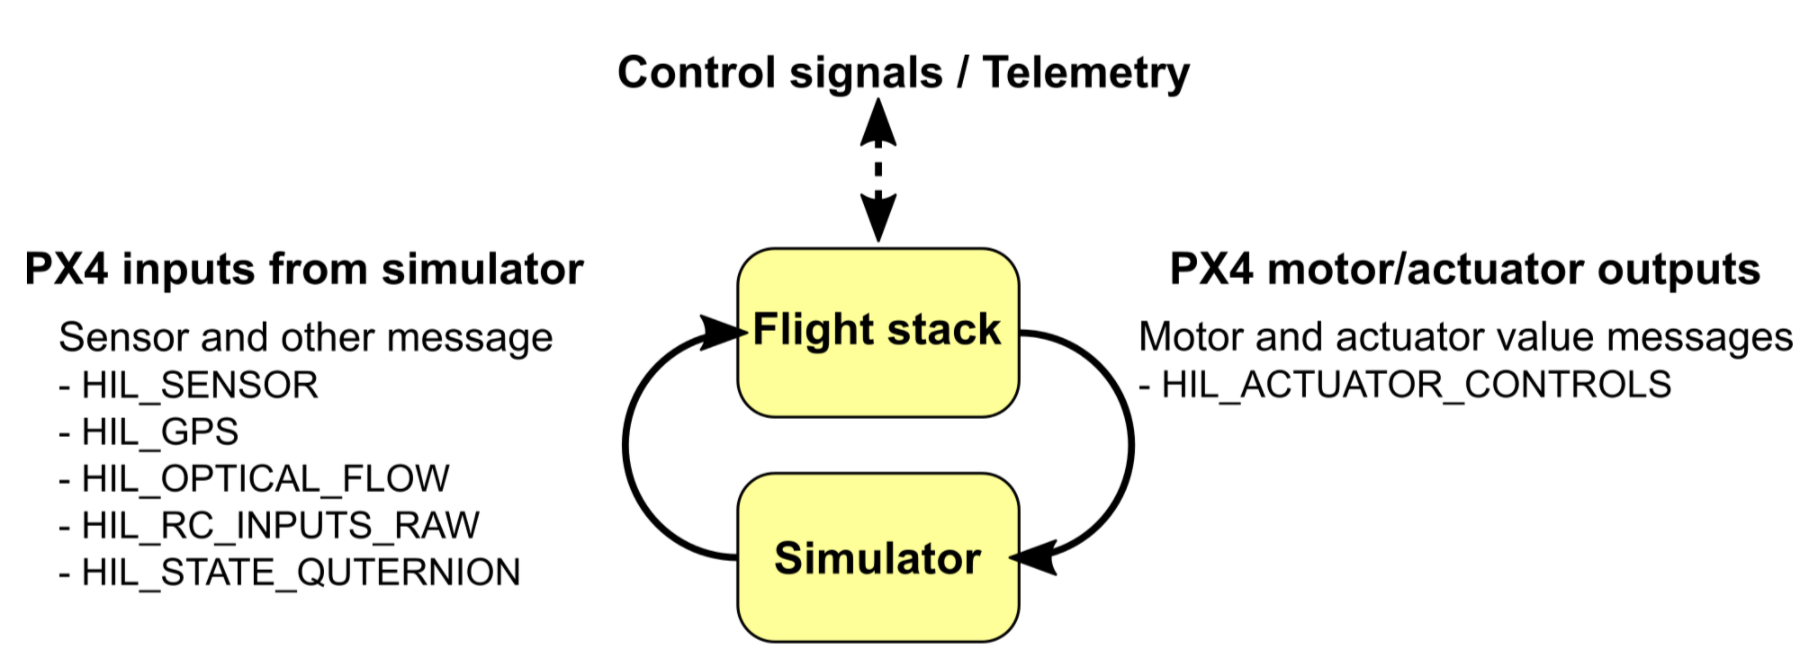
\includegraphics[scale=0.29]{obrazky/SIM1}
  \end{center}
  \caption[Tok zpráv mezi simulátorem a PX4]{Tok zpráv mezi simulátorem a PX4 \cite{SIM}.}
  \label{fig:SIM1}
\end{figure}

\section{SITL simulační prostředí}

\textit{\acl{SITL}} simulace umožňuje rychlé a \uv{levné} ladění robotických misí, protože pro simulaci \acs{SITL} se nevyužívá žádný specializovaný hardware, ale jenom počítač s nainstalovaným simulačním prostředím.

Obrázek \ref{fig:SIM2} zobrazuje typické prostředí simulace SITL v PX4 pro kterýkoliv z podporovaných simulátorů. Simulátor a PX4 firmawe mohou spolu komunikovat pomocí MAVLink \acs{API}. Pro přímou interakci s PX4 se využívá komunikace přes \textit{Micro-RTPS bridge}, kde se komunikují přímo uORB zprávy.

Různé části simulačního prostředí spolu komunikují pomocí \acs{UDP} (\acl{UDP}) a mohou být spuštěny na stejném počítači, nebo jiném počítači ve stejné síti. Pomocí sériové komunikace je možné připojit joystick, gamepad nebo RC soupravu pro ruční ovládání simulovaného dronu přes QGroundControl.

\begin{figure}[!ht]
  \begin{center}
    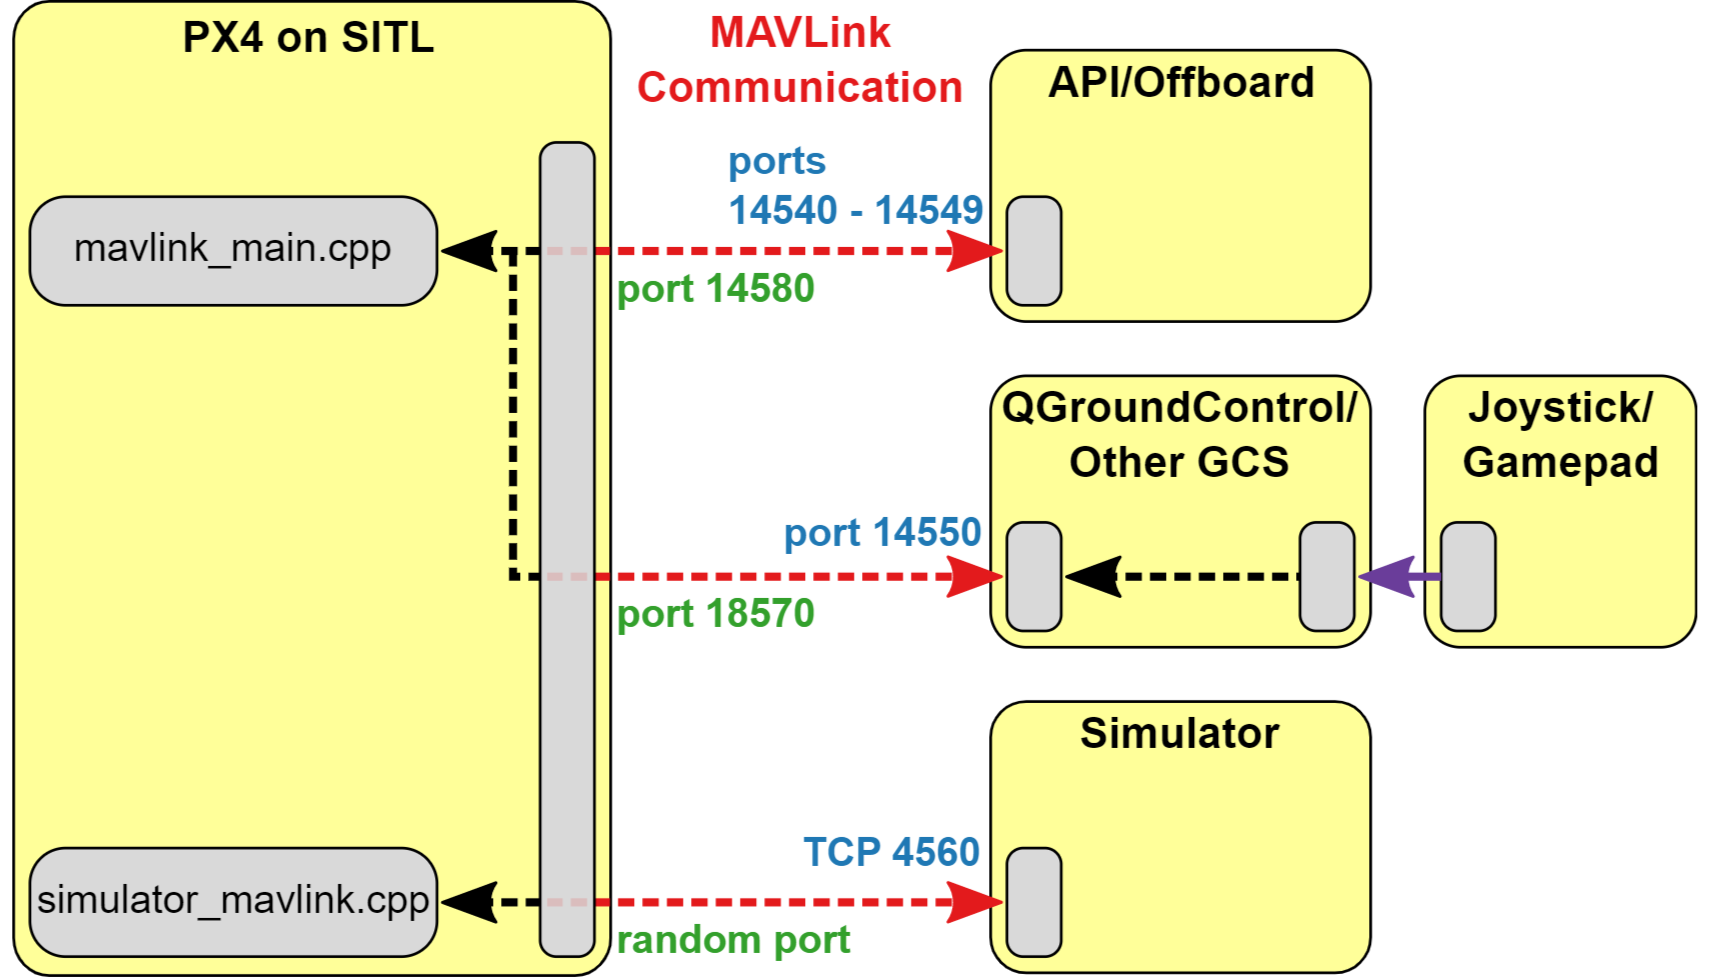
\includegraphics[scale=0.3]{obrazky/SIM2}
  \end{center}
  \caption[Diagram komunikace mezi PX4 a simulátorem]{Diagram komunikace mezi PX4 a simulátorem \cite{SIM}.}
  \label{fig:SIM2}
\end{figure}

\subsection{Seznam podporovaných simulátorů}

Následující simulátory jsou podporovány systémem PX4:

\begin{itemize}
    \item Gazebo
    \item FlightGear
    \item JSBSim
    \item jMAVSim
    \item AirSim
    \item Ignition Gazebo
\end{itemize}

\subsection{Gazebo}

Simulátor Gazebo je vysoce doporučen pro PX4 simulaci.

Gazebo je dobře navržený a otestovaný simulátor, umožňující rychlé testování algoritmů, návrh robotů a trénování systémů s umělou inteligencí v realistických scénářích. Nabízí možnost přesně a efektivně simulovat populace robotů ve složitých vnitřních i venkovních prostředích. Gazebo se běžně používá pro práci s ROS (ROS 2). \cite{GAZ}

Podporovaná vozidla \acs{SITL} simulace PX4 v simulátoru Gazebo jsou:

\begin{itemize}
    \item dron
    \item delta \acs{VTOL} (\acl{VTOL})
    \item letadlo
    \item rover
    \item ponorka
\end{itemize}

\subsection{Ignition Gazebo}

Vývojový tím simulátoru Gazebo se v budoucnu zaměří na vývoj simulátoru Ignition, takže Gazebo 11 je poslední verze známého simulátoru Gazebo. Oba simulátory jsou kompatibilní ve formátu popisu prostředí (\uv{světa}) a některých pluginů. \cite{IGN}

Z důvodu, že simulační firmware PX4 je v této době lépe propojený se simulátorem Gazebo, tak v této práci budeme pracovat s simulátorem Gazebo 11.

Jediné vozidlo, které je podporované \acs{SITL} simulací PX4 v simulátoru Ignition je dron.

\section{Instalace virtuálního prostředí}

Pro vývoj a simulaci bezpilotních misí v prostředí PX4 a ROS 2 je nutné nainstalovat jednotlivé komponenty vývojového prostředí:

\begin{itemize}
    \item PX4 simulační firmware
    \item Gazebo simulátor
    \item ROS 2 Foxy
    \item PX4 - ROS 2 \textit{bridge} (komunikační most mezi PX4 firmware a ROS 2)\\
\end{itemize}

V následujících podkapitolách si popíšeme instalaci jednotlivých částí. Návod je určený pro linuxovou distribuci Ubuntu 20.04 \textit{Focal Fossa}.

\subsection{Instalace PX4 simulačního prostředí}

Prvním krokem je instalace PX4 prostředí. Při reální misi (nebo \acs{HITL} simulaci) bude PX4 firmware spuštěný přímo na řídící jednotce Pixhawk. Při \acs{SITL} simulaci je nutné PX4 letový kód nainstalovat na počítač. Doporučená platforma pro PX4 prostředí je Ubuntu, ale je možné ho spustit na Windows 10 nebo na Mac OS.

Samotná instalace prostředí PX4 je jednoduchá a skládá se z 2 kroků. \cite{INSTALL1}

\begin{lstlisting}[language=bash]
# 1. Stáhnout zdrojový kód PX4:
$ git clone https://github.com/PX4/PX4-Autopilot.git --recursive
 
# 2. Spustit script ubuntu.sh bez argumentů
# pro instalaci všech závislostí
$ bash ./PX4-Autopilot/Tools/setup/ubuntu.sh
\end{lstlisting}

Script \texttt{ubuntu.sh} nastaví vývojové prostředí PX4, dále nainstaluje simulátory Gazebo a jMavSim a sadu nástrojů \textit{NuttX}\footnote{NuttX je \acs{RTOS} (\acl{RTOS}) pro provoz PX4 na řídící jednotce Pixhawk. Je to open source (BSD licence), lehký, výkonný a velmi stabilní operační systém. \cite{PX4main}}/\textit{Pixhawk}

\subsection{Instalace ROS 2 Foxy}

Instalace ROS 2 je dobře popsaná na dokumentačních stránkách \cite{ROS2INSTALL}. Po úspěšné instalaci ROS 2 Foxy je nutné doinstalovat několik závislostí:

\begin{lstlisting}[language=bash]
# 1. Instalační proces ROS 2 by měl nainstalovat 
# nástroje pro sestavení colcon, ale v případě, 
# že se tak nestane, můžete nástroje nainstalovat ručně:
$ sudo apt install python3-colcon-common-extensions
 
# 2. Eigen3 se používá v knihovně transformací:
$ sudo apt install ros-foxy-eigen3-cmake-module
 
# 3. Závislosti Pythonu musí být také nainstalovány:
$ sudo pip3 install -U empy pyros-genmsg setuptools
\end{lstlisting}

\subsection{Nastavení ROS 2 prostředí}

Pro vytvoření ROS 2 pracovního prostoru (\textit{workspace}) podporujícího simulaci v PX4 je nutné stáhnout dva ROS 2 balíčky. \cite{ROS2BRIDGE}

Na stáhnutí a sestavení obou balíčků můžeme použít tyto příkazy:

\begin{lstlisting}[language=bash]
# Naklonování obou balíčků:
$ mkdir -p ~/px4_ros_com_ros2/src
$ git clone https://github.com/PX4/px4_ros_com.git \
  ~/px4_ros_com_ros2/src/px4_ros_com
$ git clone https://github.com/PX4/px4_msgs.git \
  ~/px4_ros_com_ros2/src/px4_msgs
  
# Balíček px4_ros_com obsahuje scripty na sestavení workspace:
$ cd ~/px4_ros_com_ros2/src/px4_ros_com/scripts
$ source build_ros2_workspace.bash
\end{lstlisting}

\subsubsection{Balíček \texttt{px4\_msgs}}

V balíčku \texttt{px4\_msgs} je nadefinovaných víc jak 200 uORB zpráv pro komunikaci mezi ROS 2 \textit{node} a PX4 firmware.

\subsubsection{Balíček \texttt{px4\_ros\_com}}

Balíček \texttt{px4\_ros\_com} generuje přepojení mezi ROS 2 a PX4 firmware pomocí Fast RTPS (\acs{DDS}). V tomto balíčku je možné vytvářet ROS 2 misi pro autonomní řízení dronu.

\subsection{PX4 - ROS 2 bridge}

Jak je popsáno v kapitole \ref{sec:komunikace} \nameref{sec:komunikace}, pro komunikaci mezi ROS 2 \textit{node} a PX4 slouží \textit{eProsima Fast DDS}, který umožňuje výměnu zpráv uORB mezi PX4 a ROS 2.\\

Pro nastavení PX4 - ROS 2 \textit{bridge} potřebujeme nainstalovat následující balíčky:

\begin{itemize}
    \item Java JDK (Open source JDK 11)
    \item Gradle
    \item Fast-RTPS-Gen
\end{itemize}

\subsubsection{Java JDK a Gradle}

Java JDK a Gradle jsou nutné závislosti pro správnou funkci Fast-RTPS-Gen. Pro instalaci je možné použít návod zveřejněný zde: 

\href{https://linuxize.com/post/how-to-install-gradle-on-ubuntu-20-04/}{https://linuxize.com/post/how-to-install-gradle-on-ubuntu-20-04/} \cite{GRADLE}.

\subsubsection{Fast RTPS Gen}

Fast-RTPS-Gen je nástroj pro generování \acs{IDL} (\acl{IDL}) kódu pro Fast RTPS (\acs{DDS}).

Fast-RTPS-Gen je možné nainstalovat pomocí následujícího příkazu \cite{DDSGEN}:

\begin{lstlisting}[language=bash]
git clone --recursive https://github.com/eProsima/Fast-DDS-Gen.git \
    -b v1.0.4 ~/Fast-RTPS-Gen \
    && cd ~/Fast-RTPS-Gen \
    && gradle assemble \
    && sudo env "PATH=$PATH" gradle install
\end{lstlisting}

\acs{RTPS} agent se na palubním počítači spouští pomocí příkazu:

\begin{lstlisting}[language=bash]
$ source ~/px4_ros_com_ros2/install/setup.bash
$ micrortps_agent -t UDP
\end{lstlisting}

\section{ROS 2 misie}

Jedna možnost pro vytvoření autonomní mise v systému PX4 je pomocí programu QGroundControl, jak je popsáno v kapitole \ref{subs:planovani} \nameref{subs:planovani}. Zde je možné vytvořit jednoduché mise na průzkum prostředí, skenování koridoru, skenování konstrukcí a obecnou misi pomocí \textit{waypoints}. Celá mise musí být naplánovaná před startem, takže dron nemůže pohotově reagovat na různé situace, které nastanou v průběhu letu. 

Další možnost je vytvoření bezpilotní robotické mise v nadřazeném palubním počítači pomocí ROS 2 \textit{node}, který úkoluje řídící jednotku dronu. Tato možnost je vhodná pro složité mise, kde není před startem známá celá trajektorie letu a řídící algoritmus v palubním počítači ji dopočítává na základě čtení ze snímačů a kamer, nebo na základě povelů z pozemní stanice.

Pro tento případ jsme vytvořili ROS 2 \textit{node} (v C++), který komunikuje s PX4 firmware přes Fast RTPS. Zdrojový kód je zveřejněný na platformě GitHub \cite{GIT}.

Pro ovládání dronu z palubního počítače musí mít dron aktivovaný \textit{offboard flight mode} (mimopalubní letový režim).

\subsection{Offboard flight mode}

\textit{Offboard flight mode} se využívá vždy, když je dron řízený z jiného zdroje, než z Pixhawk řídící jednotky (PX4 firmware) například z palubního počítače. 

V \textit{offboard} letovém režimu se dronu posílají hlavě zprávy pro let na definovanou pozici (absolutní nebo relativní) a let určitým azimutem a rychlostí. Je vhodné, aby se pro kritické operace jako jsou vzlet, přistání, návrat na startovací pozici (\textit{Return to Launch}) využívali odpovídající letecké režimy.

Aby zůstal \textit{offboard} letový režim aktivní, palubní počítač musí posílat zprávu o aktivitě módu (\texttt{OffboardControlMode message}) s frekvencí > 2 Hz. V případě poruchy pablubního počítače, nebo nedostatečné rychlosti posílání zpráv se \textit{offboard} letový režim vypne a bude aktivovaný \textit{land} letový režim, takže dron přistane na daném místě. \cite{OFFBOADR}

\subsection{Výsledky simulace}

Pomocí ROS 2 \textit{node} se nám podařilo posílat zprávy do simulovaného PX4 firmware a tím ovládat dron v \textit{offboard} letovém režimu. Na obrázku \ref{fig:SIM3} v levém horním rohu je zobrazené, že dron je v režimu \textit{offboard flight mode}. Obrázek \ref{fig:SIM4} zobrazuje simulační prostředí Gazebo 11 které poskytuje fyzikální model \uv{světa} a graficky zobrazuje aktuální stav objektů v robotické misi.

\begin{figure}[!ht]
  \begin{center}
    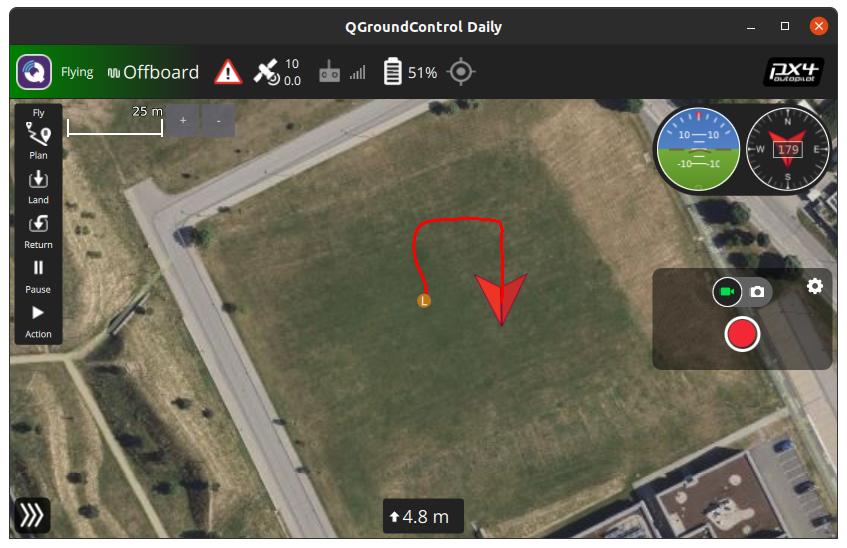
\includegraphics[scale=0.43]{obrazky/SIM3}
  \end{center}
  \caption[Software QGroundControl s dronem v \textit{offboard flight mode}]{Software QGroundControl s dronem v \textit{offboard flight mode}.}
  \label{fig:SIM3}
\end{figure}

\begin{figure}[!ht]
  \begin{center}
    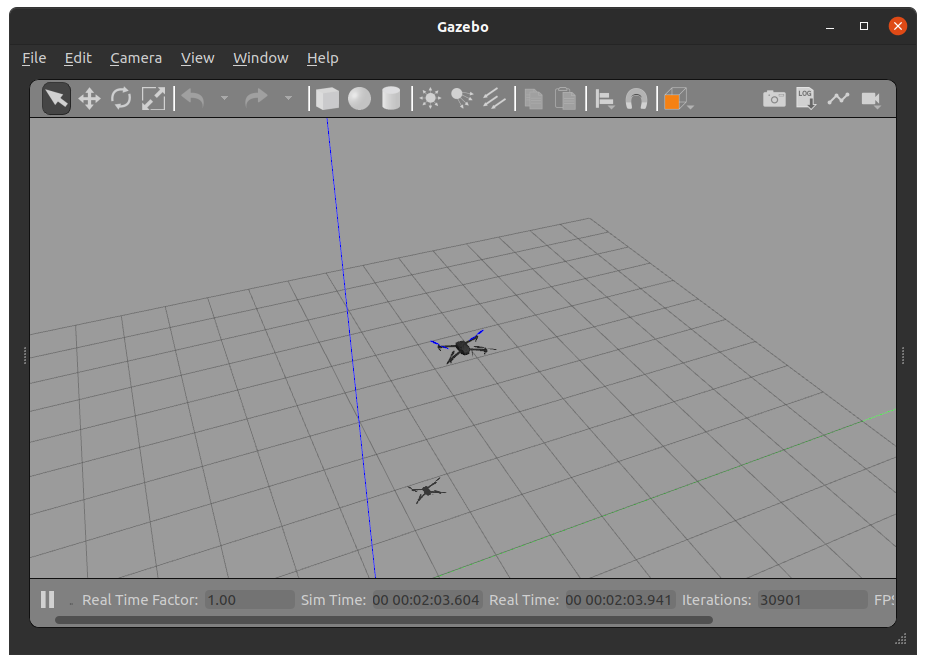
\includegraphics[scale=0.4]{obrazky/SIM4}
  \end{center}
  \caption[Bezpilotní mise v simulátoru Gazebo]{Bezpilotní mise v simulátoru Gazebo.}
  \label{fig:SIM4}
\end{figure}